\documentclass[1p]{elsarticle_modified}
%\bibliographystyle{elsarticle-num}

%\usepackage[colorlinks]{hyperref}
%\usepackage{abbrmath_seonhwa} %\Abb, \Ascr, \Acal ,\Abf, \Afrak
\usepackage{amsfonts}
\usepackage{amssymb}
\usepackage{amsmath}
\usepackage{amsthm}
\usepackage{scalefnt}
\usepackage{amsbsy}
\usepackage{kotex}
\usepackage{caption}
\usepackage{subfig}
\usepackage{color}
\usepackage{graphicx}
\usepackage{xcolor} %% white, black, red, green, blue, cyan, magenta, yellow
\usepackage{float}
\usepackage{setspace}
\usepackage{hyperref}

\usepackage{tikz}
\usetikzlibrary{arrows}

\usepackage{multirow}
\usepackage{array} % fixed length table
\usepackage{hhline}

%%%%%%%%%%%%%%%%%%%%%
\makeatletter
\renewcommand*\env@matrix[1][\arraystretch]{%
	\edef\arraystretch{#1}%
	\hskip -\arraycolsep
	\let\@ifnextchar\new@ifnextchar
	\array{*\c@MaxMatrixCols c}}
\makeatother %https://tex.stackexchange.com/questions/14071/how-can-i-increase-the-line-spacing-in-a-matrix
%%%%%%%%%%%%%%%

\usepackage[normalem]{ulem}

\newcommand{\msout}[1]{\ifmmode\text{\sout{\ensuremath{#1}}}\else\sout{#1}\fi}
%SOURCE: \msout is \stkout macro in https://tex.stackexchange.com/questions/20609/strikeout-in-math-mode

\newcommand{\cancel}[1]{
	\ifmmode
	{\color{red}\msout{#1}}
	\else
	{\color{red}\sout{#1}}
	\fi
}

\newcommand{\add}[1]{
	{\color{blue}\uwave{#1}}
}

\newcommand{\replace}[2]{
	\ifmmode
	{\color{red}\msout{#1}}{\color{blue}\uwave{#2}}
	\else
	{\color{red}\sout{#1}}{\color{blue}\uwave{#2}}
	\fi
}

\newcommand{\Sol}{\mathcal{S}} %segment
\newcommand{\D}{D} %diagram
\newcommand{\A}{\mathcal{A}} %arc


%%%%%%%%%%%%%%%%%%%%%%%%%%%%%5 test

\def\sl{\operatorname{\textup{SL}}(2,\Cbb)}
\def\psl{\operatorname{\textup{PSL}}(2,\Cbb)}
\def\quan{\mkern 1mu \triangleright \mkern 1mu}

\theoremstyle{definition}
\newtheorem{thm}{Theorem}[section]
\newtheorem{prop}[thm]{Proposition}
\newtheorem{lem}[thm]{Lemma}
\newtheorem{ques}[thm]{Question}
\newtheorem{cor}[thm]{Corollary}
\newtheorem{defn}[thm]{Definition}
\newtheorem{exam}[thm]{Example}
\newtheorem{rmk}[thm]{Remark}
\newtheorem{alg}[thm]{Algorithm}

\newcommand{\I}{\sqrt{-1}}
\begin{document}

%\begin{frontmatter}
%
%\title{Boundary parabolic representations of knots up to 8 crossings}
%
%%% Group authors per affiliation:
%\author{Yunhi Cho} 
%\address{Department of Mathematics, University of Seoul, Seoul, Korea}
%\ead{yhcho@uos.ac.kr}
%
%
%\author{Seonhwa Kim} %\fnref{s_kim}}
%\address{Center for Geometry and Physics, Institute for Basic Science, Pohang, 37673, Korea}
%\ead{ryeona17@ibs.re.kr}
%
%\author{Hyuk Kim}
%\address{Department of Mathematical Sciences, Seoul National University, Seoul 08826, Korea}
%\ead{hyukkim@snu.ac.kr}
%
%\author{Seokbeom Yoon}
%\address{Department of Mathematical Sciences, Seoul National University, Seoul, 08826,  Korea}
%\ead{sbyoon15@snu.ac.kr}
%
%\begin{abstract}
%We find all boundary parabolic representation of knots up to 8 crossings.
%
%\end{abstract}
%\begin{keyword}
%    \MSC[2010] 57M25 
%\end{keyword}
%
%\end{frontmatter}

%\linenumbers
%\tableofcontents
%
\newcommand\colored[1]{\textcolor{white}{\rule[-0.35ex]{0.8em}{1.4ex}}\kern-0.8em\color{red} #1}%
%\newcommand\colored[1]{\textcolor{white}{ #1}\kern-2.17ex	\textcolor{white}{ #1}\kern-1.81ex	\textcolor{white}{ #1}\kern-2.15ex\color{red}#1	}

{\Large $\underline{12a_{0513}~(K12a_{0513})}$}

\setlength{\tabcolsep}{10pt}
\renewcommand{\arraystretch}{1.6}
\vspace{1cm}\begin{tabular}{m{100pt}>{\centering\arraybackslash}m{274pt}}
\multirow{5}{120pt}{
	\centering
	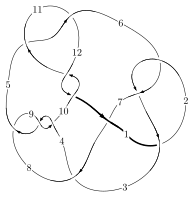
\includegraphics[width=112pt]{../../../GIT/diagram.site/Diagrams/png/1314_12a_0513.png}\\
\ \ \ A knot diagram\footnotemark}&
\allowdisplaybreaks
\textbf{Linearized knot diagam} \\
\cline{2-2}
 &
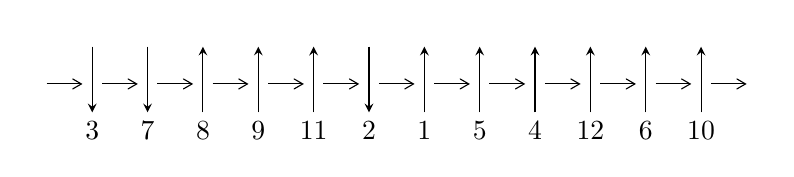
\begin{tikzpicture}[x=20pt, y=17pt]
	% nodes
	\node (C0) at (0, 0) {};
	\node (C1) at (1, 0) {};
	\node (C1U) at (1, +1) {};
	\node (C1D) at (1, -1) {3};

	\node (C2) at (2, 0) {};
	\node (C2U) at (2, +1) {};
	\node (C2D) at (2, -1) {7};

	\node (C3) at (3, 0) {};
	\node (C3U) at (3, +1) {};
	\node (C3D) at (3, -1) {8};

	\node (C4) at (4, 0) {};
	\node (C4U) at (4, +1) {};
	\node (C4D) at (4, -1) {9};

	\node (C5) at (5, 0) {};
	\node (C5U) at (5, +1) {};
	\node (C5D) at (5, -1) {11};

	\node (C6) at (6, 0) {};
	\node (C6U) at (6, +1) {};
	\node (C6D) at (6, -1) {2};

	\node (C7) at (7, 0) {};
	\node (C7U) at (7, +1) {};
	\node (C7D) at (7, -1) {1};

	\node (C8) at (8, 0) {};
	\node (C8U) at (8, +1) {};
	\node (C8D) at (8, -1) {5};

	\node (C9) at (9, 0) {};
	\node (C9U) at (9, +1) {};
	\node (C9D) at (9, -1) {4};

	\node (C10) at (10, 0) {};
	\node (C10U) at (10, +1) {};
	\node (C10D) at (10, -1) {12};

	\node (C11) at (11, 0) {};
	\node (C11U) at (11, +1) {};
	\node (C11D) at (11, -1) {6};

	\node (C12) at (12, 0) {};
	\node (C12U) at (12, +1) {};
	\node (C12D) at (12, -1) {10};
	\node (C13) at (13, 0) {};

	% arrows
	\draw[->,>={angle 60}]
	(C0) edge (C1) (C1) edge (C2) (C2) edge (C3) (C3) edge (C4) (C4) edge (C5) (C5) edge (C6) (C6) edge (C7) (C7) edge (C8) (C8) edge (C9) (C9) edge (C10) (C10) edge (C11) (C11) edge (C12) (C12) edge (C13) ;	\draw[->,>=stealth]
	(C1U) edge (C1D) (C2U) edge (C2D) (C3D) edge (C3U) (C4D) edge (C4U) (C5D) edge (C5U) (C6U) edge (C6D) (C7D) edge (C7U) (C8D) edge (C8U) (C9D) edge (C9U) (C10D) edge (C10U) (C11D) edge (C11U) (C12D) edge (C12U) ;
	\end{tikzpicture} \\
\hhline{~~} \\& 
\textbf{Solving Sequence} \\ \cline{2-2} 
 &
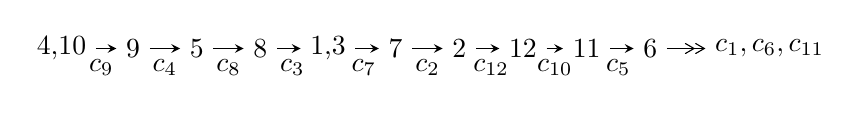
\begin{tikzpicture}[x=23pt, y=7pt]
	% node
	\node (A0) at (-1/8, 0) {4,10};
	\node (A1) at (1, 0) {9};
	\node (A2) at (2, 0) {5};
	\node (A3) at (3, 0) {8};
	\node (A4) at (65/16, 0) {1,3};
	\node (A5) at (41/8, 0) {7};
	\node (A6) at (49/8, 0) {2};
	\node (A7) at (57/8, 0) {12};
	\node (A8) at (65/8, 0) {11};
	\node (A9) at (73/8, 0) {6};
	\node (C1) at (1/2, -1) {$c_{9}$};
	\node (C2) at (3/2, -1) {$c_{4}$};
	\node (C3) at (5/2, -1) {$c_{8}$};
	\node (C4) at (7/2, -1) {$c_{3}$};
	\node (C5) at (37/8, -1) {$c_{7}$};
	\node (C6) at (45/8, -1) {$c_{2}$};
	\node (C7) at (53/8, -1) {$c_{12}$};
	\node (C8) at (61/8, -1) {$c_{10}$};
	\node (C9) at (69/8, -1) {$c_{5}$};
	\node (A10) at (11, 0) {$c_{1},c_{6},c_{11}$};

	% edge
	\draw[->,>=stealth]	
	(A0) edge (A1) (A1) edge (A2) (A2) edge (A3) (A3) edge (A4) (A4) edge (A5) (A5) edge (A6) (A6) edge (A7) (A7) edge (A8) (A8) edge (A9) ;
	\draw[->>,>={angle 60}]	
	(A9) edge (A10);
\end{tikzpicture} \\ 

\end{tabular} \\

\footnotetext{
The image of knot diagram is generated by the software ``\textbf{Draw programme}" developed by Andrew Bartholomew(\url{http://www.layer8.co.uk/maths/draw/index.htm\#Running-draw}), where we modified some parts for our purpose(\url{https://github.com/CATsTAILs/LinksPainter}).
}\phantom \\ \newline 
\centering \textbf{Ideals for irreducible components\footnotemark of $X_{\text{par}}$} 
 
\begin{align*}
I^u_{1}&=\langle 
1.92594\times10^{42} u^{79}-6.66950\times10^{42} u^{78}+\cdots+7.86358\times10^{42} b-2.35601\times10^{43},\\
\phantom{I^u_{1}}&\phantom{= \langle  }5.36807\times10^{42} u^{79}-2.27727\times10^{43} u^{78}+\cdots+7.86358\times10^{42} a-1.74971\times10^{44},\;u^{80}-4 u^{79}+\cdots-52 u+4\rangle \\
I^u_{2}&=\langle 
- a u+b+1,\;a^2+a u-1,\;u^2+1\rangle \\
I^u_{3}&=\langle 
-602 a^4 u^2-112 a^3 u^2+\cdots-678 a+1654,\\
\phantom{I^u_{3}}&\phantom{= \langle  }2 a^4 u^2+a^5+2 a^4 u+4 a^4-3 a^3 u-8 a^2 u^2-3 a^3-6 a^2 u+5 u^2 a-12 a^2+4 a u+11 u^2+9 a+5 u+18,\\
\phantom{I^u_{3}}&\phantom{= \langle  }u^3+u^2+2 u+1\rangle \\
I^u_{4}&=\langle 
a u+b,\;a^2+a u-1,\;u^2+1\rangle \\
\\
\end{align*}
\raggedright * 4 irreducible components of $\dim_{\mathbb{C}}=0$, with total 103 representations.\\
\footnotetext{All coefficients of polynomials are rational numbers. But the coefficients are sometimes approximated in decimal forms when there is not enough margin.}
\newpage
\renewcommand{\arraystretch}{1}
\centering \section*{I. $I^u_{1}= \langle 1.93\times10^{42} u^{79}-6.67\times10^{42} u^{78}+\cdots+7.86\times10^{42} b-2.36\times10^{43},\;5.37\times10^{42} u^{79}-2.28\times10^{43} u^{78}+\cdots+7.86\times10^{42} a-1.75\times10^{44},\;u^{80}-4 u^{79}+\cdots-52 u+4 \rangle$}
\flushleft \textbf{(i) Arc colorings}\\
\begin{tabular}{m{7pt} m{180pt} m{7pt} m{180pt} }
\flushright $a_{4}=$&$\begin{pmatrix}0\\u\end{pmatrix}$ \\
\flushright $a_{10}=$&$\begin{pmatrix}1\\0\end{pmatrix}$ \\
\flushright $a_{9}=$&$\begin{pmatrix}1\\u^2\end{pmatrix}$ \\
\flushright $a_{5}=$&$\begin{pmatrix}u\\u^3+u\end{pmatrix}$ \\
\flushright $a_{8}=$&$\begin{pmatrix}u^2+1\\u^4+2 u^2\end{pmatrix}$ \\
\flushright $a_{1}=$&$\begin{pmatrix}-0.682650 u^{79}+2.89597 u^{78}+\cdots-176.929 u+22.2508\\-0.244918 u^{79}+0.848150 u^{78}+\cdots-31.1691 u+2.99611\end{pmatrix}$ \\
\flushright $a_{3}=$&$\begin{pmatrix}- u^5-2 u^3- u\\- u^7-3 u^5-2 u^3+u\end{pmatrix}$ \\
\flushright $a_{7}=$&$\begin{pmatrix}0.284048 u^{79}-1.00384 u^{78}+\cdots+100.169 u-16.0275\\0.259001 u^{79}-1.01996 u^{78}+\cdots+36.9256 u-4.27465\end{pmatrix}$ \\
\flushright $a_{2}=$&$\begin{pmatrix}-0.595274 u^{79}+2.67307 u^{78}+\cdots-170.692 u+21.3726\\-0.245575 u^{79}+0.838980 u^{78}+\cdots-34.0566 u+3.54660\end{pmatrix}$ \\
\flushright $a_{12}=$&$\begin{pmatrix}-0.437731 u^{79}+2.04782 u^{78}+\cdots-145.760 u+19.2547\\-0.244918 u^{79}+0.848150 u^{78}+\cdots-31.1691 u+2.99611\end{pmatrix}$ \\
\flushright $a_{11}=$&$\begin{pmatrix}0.211687 u^{79}-0.839912 u^{78}+\cdots+3.89957 u+5.74577\\-0.381115 u^{79}+1.41021 u^{78}+\cdots-36.1654 u+4.19766\end{pmatrix}$ \\
\flushright $a_{6}=$&$\begin{pmatrix}1.04592 u^{79}-4.04767 u^{78}+\cdots+105.753 u-6.02938\\-0.123990 u^{79}+0.478152 u^{78}+\cdots-0.617434 u+1.20681\end{pmatrix}$\\&\end{tabular}
\flushleft \textbf{(ii) Obstruction class $= -1$}\\~\\
\flushleft \textbf{(iii) Cusp Shapes $= -2.35269 u^{79}+7.88005 u^{78}+\cdots-272.741 u+41.4718$}\\~\\
\newpage\renewcommand{\arraystretch}{1}
\flushleft \textbf{(iv) u-Polynomials at the component}\newline \\
\begin{tabular}{m{50pt}|m{274pt}}
Crossings & \hspace{64pt}u-Polynomials at each crossing \\
\hline $$\begin{aligned}c_{1}\end{aligned}$$&$\begin{aligned}
&u^{80}+39 u^{79}+\cdots+6 u+1
\end{aligned}$\\
\hline $$\begin{aligned}c_{2},c_{6}\end{aligned}$$&$\begin{aligned}
&u^{80}- u^{79}+\cdots-3 u^2+1
\end{aligned}$\\
\hline $$\begin{aligned}c_{3}\end{aligned}$$&$\begin{aligned}
&u^{80}-4 u^{79}+\cdots+16384 u+1024
\end{aligned}$\\
\hline $$\begin{aligned}c_{4},c_{8},c_{9}\end{aligned}$$&$\begin{aligned}
&u^{80}+4 u^{79}+\cdots+52 u+4
\end{aligned}$\\
\hline $$\begin{aligned}c_{5},c_{11}\end{aligned}$$&$\begin{aligned}
&u^{80}- u^{79}+\cdots+6 u+1
\end{aligned}$\\
\hline $$\begin{aligned}c_{7}\end{aligned}$$&$\begin{aligned}
&u^{80}-3 u^{79}+\cdots+1122 u+989
\end{aligned}$\\
\hline $$\begin{aligned}c_{10},c_{12}\end{aligned}$$&$\begin{aligned}
&u^{80}-27 u^{79}+\cdots-22 u+1
\end{aligned}$\\
\hline
\end{tabular}\\~\\
\newpage\renewcommand{\arraystretch}{1}
\flushleft \textbf{(v) Riley Polynomials at the component}\newline \\
\begin{tabular}{m{50pt}|m{274pt}}
Crossings & \hspace{64pt}Riley Polynomials at each crossing \\
\hline $$\begin{aligned}c_{1}\end{aligned}$$&$\begin{aligned}
&y^{80}+9 y^{79}+\cdots+18 y+1
\end{aligned}$\\
\hline $$\begin{aligned}c_{2},c_{6}\end{aligned}$$&$\begin{aligned}
&y^{80}-39 y^{79}+\cdots-6 y+1
\end{aligned}$\\
\hline $$\begin{aligned}c_{3}\end{aligned}$$&$\begin{aligned}
&y^{80}-20 y^{79}+\cdots-70254592 y+1048576
\end{aligned}$\\
\hline $$\begin{aligned}c_{4},c_{8},c_{9}\end{aligned}$$&$\begin{aligned}
&y^{80}+68 y^{79}+\cdots-632 y+16
\end{aligned}$\\
\hline $$\begin{aligned}c_{5},c_{11}\end{aligned}$$&$\begin{aligned}
&y^{80}-27 y^{79}+\cdots-22 y+1
\end{aligned}$\\
\hline $$\begin{aligned}c_{7}\end{aligned}$$&$\begin{aligned}
&y^{80}+21 y^{79}+\cdots+14907310 y+978121
\end{aligned}$\\
\hline $$\begin{aligned}c_{10},c_{12}\end{aligned}$$&$\begin{aligned}
&y^{80}+57 y^{79}+\cdots-54 y+1
\end{aligned}$\\
\hline
\end{tabular}\\~\\
\newpage\flushleft \textbf{(vi) Complex Volumes and Cusp Shapes}
$$\begin{array}{c|c|c}  
\text{Solutions to }I^u_{1}& \I (\text{vol} + \sqrt{-1}CS) & \text{Cusp shape}\\
 \hline 
\begin{aligned}
u &= -0.551136 + 0.802488 I \\
a &= \phantom{-}0.554036 - 0.632918 I \\
b &= -0.296637 - 1.259010 I\end{aligned}
 & -4.73746 + 0.08999 I & \phantom{-0.000000 } 0 \\ \hline\begin{aligned}
u &= -0.551136 - 0.802488 I \\
a &= \phantom{-}0.554036 + 0.632918 I \\
b &= -0.296637 + 1.259010 I\end{aligned}
 & -4.73746 - 0.08999 I & \phantom{-0.000000 } 0 \\ \hline\begin{aligned}
u &= -0.208379 + 1.008740 I \\
a &= \phantom{-}0.1249350 - 0.0323541 I \\
b &= -0.226657 + 0.715830 I\end{aligned}
 & -1.88182 - 2.17157 I & \phantom{-0.000000 } 0 \\ \hline\begin{aligned}
u &= -0.208379 - 1.008740 I \\
a &= \phantom{-}0.1249350 + 0.0323541 I \\
b &= -0.226657 - 0.715830 I\end{aligned}
 & -1.88182 + 2.17157 I & \phantom{-0.000000 } 0 \\ \hline\begin{aligned}
u &= -0.106567 + 1.055930 I \\
a &= \phantom{-}0.842709 - 0.235495 I \\
b &= -0.0559371 + 0.0534132 I\end{aligned}
 & -1.50643 - 2.08258 I & \phantom{-0.000000 } 0 \\ \hline\begin{aligned}
u &= -0.106567 - 1.055930 I \\
a &= \phantom{-}0.842709 + 0.235495 I \\
b &= -0.0559371 - 0.0534132 I\end{aligned}
 & -1.50643 + 2.08258 I & \phantom{-0.000000 } 0 \\ \hline\begin{aligned}
u &= \phantom{-}0.596084 + 0.710997 I \\
a &= -0.493767 - 0.447695 I \\
b &= -0.163120 - 1.208000 I\end{aligned}
 & -4.92608 + 5.37940 I & \phantom{-0.000000 } 0 \\ \hline\begin{aligned}
u &= \phantom{-}0.596084 - 0.710997 I \\
a &= -0.493767 + 0.447695 I \\
b &= -0.163120 + 1.208000 I\end{aligned}
 & -4.92608 - 5.37940 I & \phantom{-0.000000 } 0 \\ \hline\begin{aligned}
u &= \phantom{-}0.521840 + 0.938751 I \\
a &= -0.055226 - 0.427953 I \\
b &= \phantom{-}0.013258 - 1.063850 I\end{aligned}
 & -4.08872 - 1.79777 I & \phantom{-0.000000 } 0 \\ \hline\begin{aligned}
u &= \phantom{-}0.521840 - 0.938751 I \\
a &= -0.055226 + 0.427953 I \\
b &= \phantom{-}0.013258 + 1.063850 I\end{aligned}
 & -4.08872 + 1.79777 I & \phantom{-0.000000 } 0\\
 \hline 
 \end{array}$$\newpage$$\begin{array}{c|c|c}  
\text{Solutions to }I^u_{1}& \I (\text{vol} + \sqrt{-1}CS) & \text{Cusp shape}\\
 \hline 
\begin{aligned}
u &= \phantom{-}0.408175 + 1.010050 I \\
a &= \phantom{-}0.171639 + 0.544181 I \\
b &= -0.509729 + 1.240020 I\end{aligned}
 & -1.18830 - 2.70563 I & \phantom{-0.000000 } 0 \\ \hline\begin{aligned}
u &= \phantom{-}0.408175 - 1.010050 I \\
a &= \phantom{-}0.171639 - 0.544181 I \\
b &= -0.509729 - 1.240020 I\end{aligned}
 & -1.18830 + 2.70563 I & \phantom{-0.000000 } 0 \\ \hline\begin{aligned}
u &= -0.879762 + 0.227693 I \\
a &= -1.51369 + 1.09263 I \\
b &= -0.55379 + 1.42889 I\end{aligned}
 & -0.91388 - 12.22470 I & \phantom{-}6.00000 + 9.71272 I \\ \hline\begin{aligned}
u &= -0.879762 - 0.227693 I \\
a &= -1.51369 - 1.09263 I \\
b &= -0.55379 - 1.42889 I\end{aligned}
 & -0.91388 + 12.22470 I & \phantom{-}6.00000 - 9.71272 I \\ \hline\begin{aligned}
u &= \phantom{-}0.838234 + 0.262017 I \\
a &= \phantom{-}1.27745 + 0.85390 I \\
b &= \phantom{-}0.199465 + 1.029370 I\end{aligned}
 & -2.02492 + 6.59780 I & \phantom{-}3.40984 - 5.16517 I \\ \hline\begin{aligned}
u &= \phantom{-}0.838234 - 0.262017 I \\
a &= \phantom{-}1.27745 - 0.85390 I \\
b &= \phantom{-}0.199465 - 1.029370 I\end{aligned}
 & -2.02492 - 6.59780 I & \phantom{-}3.40984 + 5.16517 I \\ \hline\begin{aligned}
u &= -0.305412 + 0.799433 I \\
a &= -0.1368440 + 0.0226105 I \\
b &= -0.215314 + 0.977607 I\end{aligned}
 & -1.84711 - 2.26526 I & \phantom{-}3.71962 + 4.08071 I \\ \hline\begin{aligned}
u &= -0.305412 - 0.799433 I \\
a &= -0.1368440 - 0.0226105 I \\
b &= -0.215314 - 0.977607 I\end{aligned}
 & -1.84711 + 2.26526 I & \phantom{-}3.71962 - 4.08071 I \\ \hline\begin{aligned}
u &= -0.528719 + 1.021590 I \\
a &= \phantom{-}0.227668 - 0.723744 I \\
b &= -0.47028 - 1.34644 I\end{aligned}
 & -3.33066 + 7.25011 I & \phantom{-0.000000 } 0 \\ \hline\begin{aligned}
u &= -0.528719 - 1.021590 I \\
a &= \phantom{-}0.227668 + 0.723744 I \\
b &= -0.47028 + 1.34644 I\end{aligned}
 & -3.33066 - 7.25011 I & \phantom{-0.000000 } 0\\
 \hline 
 \end{array}$$\newpage$$\begin{array}{c|c|c}  
\text{Solutions to }I^u_{1}& \I (\text{vol} + \sqrt{-1}CS) & \text{Cusp shape}\\
 \hline 
\begin{aligned}
u &= \phantom{-}0.823129 + 0.204152 I \\
a &= -1.60401 - 1.00000 I \\
b &= -0.56137 - 1.37914 I\end{aligned}
 & \phantom{-}1.28021 + 7.17762 I & \phantom{-}8.76583 - 5.85883 I \\ \hline\begin{aligned}
u &= \phantom{-}0.823129 - 0.204152 I \\
a &= -1.60401 + 1.00000 I \\
b &= -0.56137 + 1.37914 I\end{aligned}
 & \phantom{-}1.28021 - 7.17762 I & \phantom{-}8.76583 + 5.85883 I \\ \hline\begin{aligned}
u &= -0.765302 + 0.332337 I \\
a &= -1.36288 + 0.78683 I \\
b &= -0.45279 + 1.35433 I\end{aligned}
 & -3.33691 - 4.71601 I & \phantom{-}1.93926 + 4.79761 I \\ \hline\begin{aligned}
u &= -0.765302 - 0.332337 I \\
a &= -1.36288 - 0.78683 I \\
b &= -0.45279 - 1.35433 I\end{aligned}
 & -3.33691 + 4.71601 I & \phantom{-}1.93926 - 4.79761 I \\ \hline\begin{aligned}
u &= \phantom{-}0.709218 + 0.403703 I \\
a &= \phantom{-}1.139150 + 0.747614 I \\
b &= \phantom{-}0.018638 + 1.087730 I\end{aligned}
 & -4.06181 - 0.78432 I & \phantom{-}0.213330 + 0.601164 I \\ \hline\begin{aligned}
u &= \phantom{-}0.709218 - 0.403703 I \\
a &= \phantom{-}1.139150 - 0.747614 I \\
b &= \phantom{-}0.018638 - 1.087730 I\end{aligned}
 & -4.06181 + 0.78432 I & \phantom{-}0.213330 - 0.601164 I \\ \hline\begin{aligned}
u &= -0.330389 + 1.137220 I \\
a &= -0.553942 - 1.234000 I \\
b &= -0.941219 - 0.028962 I\end{aligned}
 & \phantom{-}0.99595 + 2.18968 I & \phantom{-0.000000 } 0 \\ \hline\begin{aligned}
u &= -0.330389 - 1.137220 I \\
a &= -0.553942 + 1.234000 I \\
b &= -0.941219 + 0.028962 I\end{aligned}
 & \phantom{-}0.99595 - 2.18968 I & \phantom{-0.000000 } 0 \\ \hline\begin{aligned}
u &= -0.761131 + 0.226648 I \\
a &= \phantom{-}1.29441 - 0.79477 I \\
b &= \phantom{-}0.146142 - 0.958477 I\end{aligned}
 & \phantom{-}0.18029 - 1.72517 I & \phantom{-}6.96648 + 1.19694 I \\ \hline\begin{aligned}
u &= -0.761131 - 0.226648 I \\
a &= \phantom{-}1.29441 + 0.79477 I \\
b &= \phantom{-}0.146142 + 0.958477 I\end{aligned}
 & \phantom{-}0.18029 + 1.72517 I & \phantom{-}6.96648 - 1.19694 I\\
 \hline 
 \end{array}$$\newpage$$\begin{array}{c|c|c}  
\text{Solutions to }I^u_{1}& \I (\text{vol} + \sqrt{-1}CS) & \text{Cusp shape}\\
 \hline 
\begin{aligned}
u &= -0.769110 + 0.124508 I \\
a &= -2.01859 + 0.33682 I \\
b &= -1.140500 + 0.180943 I\end{aligned}
 & \phantom{-}4.05517 - 6.19535 I & \phantom{-}11.24164 + 6.13913 I \\ \hline\begin{aligned}
u &= -0.769110 - 0.124508 I \\
a &= -2.01859 - 0.33682 I \\
b &= -1.140500 - 0.180943 I\end{aligned}
 & \phantom{-}4.05517 + 6.19535 I & \phantom{-}11.24164 - 6.13913 I \\ \hline\begin{aligned}
u &= \phantom{-}0.220897 + 1.201700 I \\
a &= -0.221048 + 0.378026 I \\
b &= -0.755621 + 1.106820 I\end{aligned}
 & -1.01320 - 1.61452 I & \phantom{-0.000000 } 0 \\ \hline\begin{aligned}
u &= \phantom{-}0.220897 - 1.201700 I \\
a &= -0.221048 - 0.378026 I \\
b &= -0.755621 - 1.106820 I\end{aligned}
 & -1.01320 + 1.61452 I & \phantom{-0.000000 } 0 \\ \hline\begin{aligned}
u &= \phantom{-}0.763645 + 0.064433 I \\
a &= -1.96075 - 0.18144 I \\
b &= -1.126830 - 0.094815 I\end{aligned}
 & \phantom{-}5.81886 + 1.20518 I & \phantom{-}14.4550 - 0.8575 I \\ \hline\begin{aligned}
u &= \phantom{-}0.763645 - 0.064433 I \\
a &= -1.96075 + 0.18144 I \\
b &= -1.126830 + 0.094815 I\end{aligned}
 & \phantom{-}5.81886 - 1.20518 I & \phantom{-}14.4550 + 0.8575 I \\ \hline\begin{aligned}
u &= \phantom{-}0.327694 + 1.195580 I \\
a &= -0.696454 + 1.008560 I \\
b &= -1.033350 - 0.080637 I\end{aligned}
 & \phantom{-}2.36178 + 2.75003 I & \phantom{-0.000000 } 0 \\ \hline\begin{aligned}
u &= \phantom{-}0.327694 - 1.195580 I \\
a &= -0.696454 - 1.008560 I \\
b &= -1.033350 + 0.080637 I\end{aligned}
 & \phantom{-}2.36178 - 2.75003 I & \phantom{-0.000000 } 0 \\ \hline\begin{aligned}
u &= \phantom{-}0.147606 + 1.296040 I \\
a &= \phantom{-}1.63223 - 1.23495 I \\
b &= -0.037662 + 1.042620 I\end{aligned}
 & -3.72526 - 2.52051 I & \phantom{-0.000000 } 0 \\ \hline\begin{aligned}
u &= \phantom{-}0.147606 - 1.296040 I \\
a &= \phantom{-}1.63223 + 1.23495 I \\
b &= -0.037662 - 1.042620 I\end{aligned}
 & -3.72526 + 2.52051 I & \phantom{-0.000000 } 0\\
 \hline 
 \end{array}$$\newpage$$\begin{array}{c|c|c}  
\text{Solutions to }I^u_{1}& \I (\text{vol} + \sqrt{-1}CS) & \text{Cusp shape}\\
 \hline 
\begin{aligned}
u &= -0.049107 + 1.308430 I \\
a &= -0.502531 - 0.144008 I \\
b &= -0.949755 - 0.904347 I\end{aligned}
 & -4.24144 + 4.07906 I & \phantom{-0.000000 } 0 \\ \hline\begin{aligned}
u &= -0.049107 - 1.308430 I \\
a &= -0.502531 + 0.144008 I \\
b &= -0.949755 + 0.904347 I\end{aligned}
 & -4.24144 - 4.07906 I & \phantom{-0.000000 } 0 \\ \hline\begin{aligned}
u &= \phantom{-}0.670555 + 0.086690 I \\
a &= -2.05137 - 0.81648 I \\
b &= -0.613705 - 1.242710 I\end{aligned}
 & \phantom{-}2.33556 + 4.87257 I & \phantom{-}10.70507 - 5.88102 I \\ \hline\begin{aligned}
u &= \phantom{-}0.670555 - 0.086690 I \\
a &= -2.05137 + 0.81648 I \\
b &= -0.613705 + 1.242710 I\end{aligned}
 & \phantom{-}2.33556 - 4.87257 I & \phantom{-}10.70507 + 5.88102 I \\ \hline\begin{aligned}
u &= \phantom{-}0.315351 + 1.304030 I \\
a &= -0.921696 + 0.699551 I \\
b &= -1.203010 - 0.251403 I\end{aligned}
 & \phantom{-}1.54253 + 5.09315 I & \phantom{-0.000000 } 0 \\ \hline\begin{aligned}
u &= \phantom{-}0.315351 - 1.304030 I \\
a &= -0.921696 - 0.699551 I \\
b &= -1.203010 + 0.251403 I\end{aligned}
 & \phantom{-}1.54253 - 5.09315 I & \phantom{-0.000000 } 0 \\ \hline\begin{aligned}
u &= \phantom{-}0.266524 + 1.325000 I \\
a &= -1.62612 + 1.19602 I \\
b &= -0.51362 - 1.36083 I\end{aligned}
 & -2.10689 + 8.26650 I & \phantom{-0.000000 } 0 \\ \hline\begin{aligned}
u &= \phantom{-}0.266524 - 1.325000 I \\
a &= -1.62612 - 1.19602 I \\
b &= -0.51362 + 1.36083 I\end{aligned}
 & -2.10689 - 8.26650 I & \phantom{-0.000000 } 0 \\ \hline\begin{aligned}
u &= \phantom{-}0.585654 + 0.221603 I \\
a &= \phantom{-}1.32826 - 0.55799 I \\
b &= \phantom{-}0.211347 - 0.394465 I\end{aligned}
 & -0.36980 + 4.43761 I & \phantom{-}4.75087 - 6.66233 I \\ \hline\begin{aligned}
u &= \phantom{-}0.585654 - 0.221603 I \\
a &= \phantom{-}1.32826 + 0.55799 I \\
b &= \phantom{-}0.211347 + 0.394465 I\end{aligned}
 & -0.36980 - 4.43761 I & \phantom{-}4.75087 + 6.66233 I\\
 \hline 
 \end{array}$$\newpage$$\begin{array}{c|c|c}  
\text{Solutions to }I^u_{1}& \I (\text{vol} + \sqrt{-1}CS) & \text{Cusp shape}\\
 \hline 
\begin{aligned}
u &= \phantom{-}0.121476 + 1.374030 I \\
a &= \phantom{-}0.776792 - 0.099407 I \\
b &= \phantom{-}0.497170 - 0.215952 I\end{aligned}
 & -7.00972 - 0.03580 I & \phantom{-0.000000 } 0 \\ \hline\begin{aligned}
u &= \phantom{-}0.121476 - 1.374030 I \\
a &= \phantom{-}0.776792 + 0.099407 I \\
b &= \phantom{-}0.497170 + 0.215952 I\end{aligned}
 & -7.00972 + 0.03580 I & \phantom{-0.000000 } 0 \\ \hline\begin{aligned}
u &= -0.319084 + 1.344980 I \\
a &= -1.014690 - 0.624204 I \\
b &= -1.275130 + 0.292082 I\end{aligned}
 & -0.57753 - 10.12060 I & \phantom{-0.000000 } 0 \\ \hline\begin{aligned}
u &= -0.319084 - 1.344980 I \\
a &= -1.014690 + 0.624204 I \\
b &= -1.275130 - 0.292082 I\end{aligned}
 & -0.57753 + 10.12060 I & \phantom{-0.000000 } 0 \\ \hline\begin{aligned}
u &= \phantom{-}0.245398 + 1.369620 I \\
a &= \phantom{-}0.722283 - 0.225370 I \\
b &= \phantom{-}0.505471 - 0.436922 I\end{aligned}
 & -5.38272 + 7.52809 I & \phantom{-0.000000 } 0 \\ \hline\begin{aligned}
u &= \phantom{-}0.245398 - 1.369620 I \\
a &= \phantom{-}0.722283 + 0.225370 I \\
b &= \phantom{-}0.505471 + 0.436922 I\end{aligned}
 & -5.38272 - 7.52809 I & \phantom{-0.000000 } 0 \\ \hline\begin{aligned}
u &= -0.31258 + 1.39281 I \\
a &= \phantom{-}1.48142 + 0.38881 I \\
b &= \phantom{-}0.264823 - 1.069660 I\end{aligned}
 & -4.95968 - 5.61831 I & \phantom{-0.000000 } 0 \\ \hline\begin{aligned}
u &= -0.31258 - 1.39281 I \\
a &= \phantom{-}1.48142 - 0.38881 I \\
b &= \phantom{-}0.264823 + 1.069660 I\end{aligned}
 & -4.95968 + 5.61831 I & \phantom{-0.000000 } 0 \\ \hline\begin{aligned}
u &= \phantom{-}0.34340 + 1.39206 I \\
a &= -1.60088 + 0.60509 I \\
b &= -0.56567 - 1.47569 I\end{aligned}
 & -3.78107 + 11.38600 I & \phantom{-0.000000 } 0 \\ \hline\begin{aligned}
u &= \phantom{-}0.34340 - 1.39206 I \\
a &= -1.60088 - 0.60509 I \\
b &= -0.56567 + 1.47569 I\end{aligned}
 & -3.78107 - 11.38600 I & \phantom{-0.000000 } 0\\
 \hline 
 \end{array}$$\newpage$$\begin{array}{c|c|c}  
\text{Solutions to }I^u_{1}& \I (\text{vol} + \sqrt{-1}CS) & \text{Cusp shape}\\
 \hline 
\begin{aligned}
u &= -0.02337 + 1.45374 I \\
a &= \phantom{-}0.149541 - 1.005020 I \\
b &= -0.150773 + 1.367660 I\end{aligned}
 & -8.93138 - 2.93585 I & \phantom{-0.000000 } 0 \\ \hline\begin{aligned}
u &= -0.02337 - 1.45374 I \\
a &= \phantom{-}0.149541 + 1.005020 I \\
b &= -0.150773 - 1.367660 I\end{aligned}
 & -8.93138 + 2.93585 I & \phantom{-0.000000 } 0 \\ \hline\begin{aligned}
u &= -0.29501 + 1.42781 I \\
a &= -1.30790 - 0.65861 I \\
b &= -0.49197 + 1.49263 I\end{aligned}
 & -8.94290 - 8.53329 I & \phantom{-0.000000 } 0 \\ \hline\begin{aligned}
u &= -0.29501 - 1.42781 I \\
a &= -1.30790 + 0.65861 I \\
b &= -0.49197 - 1.49263 I\end{aligned}
 & -8.94290 + 8.53329 I & \phantom{-0.000000 } 0 \\ \hline\begin{aligned}
u &= \phantom{-}0.34014 + 1.41816 I \\
a &= \phantom{-}1.45611 - 0.29908 I \\
b &= \phantom{-}0.319417 + 1.089870 I\end{aligned}
 & -7.36888 + 10.84370 I & \phantom{-0.000000 } 0 \\ \hline\begin{aligned}
u &= \phantom{-}0.34014 - 1.41816 I \\
a &= \phantom{-}1.45611 + 0.29908 I \\
b &= \phantom{-}0.319417 - 1.089870 I\end{aligned}
 & -7.36888 - 10.84370 I & \phantom{-0.000000 } 0 \\ \hline\begin{aligned}
u &= \phantom{-}0.25771 + 1.43558 I \\
a &= \phantom{-}1.292160 - 0.461107 I \\
b &= \phantom{-}0.212673 + 1.164040 I\end{aligned}
 & -9.91847 + 2.66208 I & \phantom{-0.000000 } 0 \\ \hline\begin{aligned}
u &= \phantom{-}0.25771 - 1.43558 I \\
a &= \phantom{-}1.292160 + 0.461107 I \\
b &= \phantom{-}0.212673 - 1.164040 I\end{aligned}
 & -9.91847 - 2.66208 I & \phantom{-0.000000 } 0 \\ \hline\begin{aligned}
u &= -0.36648 + 1.41215 I \\
a &= -1.59384 - 0.46201 I \\
b &= -0.58244 + 1.50990 I\end{aligned}
 & -6.1192 - 16.7066 I & \phantom{-0.000000 } 0 \\ \hline\begin{aligned}
u &= -0.36648 - 1.41215 I \\
a &= -1.59384 + 0.46201 I \\
b &= -0.58244 - 1.50990 I\end{aligned}
 & -6.1192 + 16.7066 I & \phantom{-0.000000 } 0\\
 \hline 
 \end{array}$$\newpage$$\begin{array}{c|c|c}  
\text{Solutions to }I^u_{1}& \I (\text{vol} + \sqrt{-1}CS) & \text{Cusp shape}\\
 \hline 
\begin{aligned}
u &= \phantom{-}0.267652 + 0.469417 I \\
a &= \phantom{-}1.287930 - 0.150939 I \\
b &= \phantom{-}0.155923 - 0.055103 I\end{aligned}
 & -1.47309 - 1.47748 I & \phantom{-}0.853173 + 0.501389 I \\ \hline\begin{aligned}
u &= \phantom{-}0.267652 - 0.469417 I \\
a &= \phantom{-}1.287930 + 0.150939 I \\
b &= \phantom{-}0.155923 + 0.055103 I\end{aligned}
 & -1.47309 + 1.47748 I & \phantom{-}0.853173 - 0.501389 I \\ \hline\begin{aligned}
u &= -0.03028 + 1.50039 I \\
a &= \phantom{-}0.383013 + 0.722409 I \\
b &= -0.053416 - 1.393890 I\end{aligned}
 & -12.59510 - 1.27716 I & \phantom{-0.000000 } 0 \\ \hline\begin{aligned}
u &= -0.03028 - 1.50039 I \\
a &= \phantom{-}0.383013 - 0.722409 I \\
b &= -0.053416 + 1.393890 I\end{aligned}
 & -12.59510 + 1.27716 I & \phantom{-0.000000 } 0 \\ \hline\begin{aligned}
u &= \phantom{-}0.07316 + 1.49993 I \\
a &= -0.118714 + 0.762219 I \\
b &= -0.18506 - 1.45576 I\end{aligned}
 & -12.4175 + 7.3131 I & \phantom{-0.000000 } 0 \\ \hline\begin{aligned}
u &= \phantom{-}0.07316 - 1.49993 I \\
a &= -0.118714 - 0.762219 I \\
b &= -0.18506 + 1.45576 I\end{aligned}
 & -12.4175 - 7.3131 I & \phantom{-0.000000 } 0 \\ \hline\begin{aligned}
u &= -0.410317 + 0.068593 I \\
a &= \phantom{-}0.076036 + 0.775710 I \\
b &= -0.417482 + 0.255970 I\end{aligned}
 & \phantom{-}0.972335 - 0.113438 I & \phantom{-}11.49870 + 0.99619 I \\ \hline\begin{aligned}
u &= -0.410317 - 0.068593 I \\
a &= \phantom{-}0.076036 - 0.775710 I \\
b &= -0.417482 - 0.255970 I\end{aligned}
 & \phantom{-}0.972335 + 0.113438 I & \phantom{-}11.49870 - 0.99619 I \\ \hline\begin{aligned}
u &= \phantom{-}0.168606 + 0.085574 I \\
a &= \phantom{-}1.38717 - 5.08704 I \\
b &= -0.501486 - 0.738647 I\end{aligned}
 & \phantom{-}0.08992 + 4.10562 I & \phantom{-}9.80690 - 7.22475 I \\ \hline\begin{aligned}
u &= \phantom{-}0.168606 - 0.085574 I \\
a &= \phantom{-}1.38717 + 5.08704 I \\
b &= -0.501486 + 0.738647 I\end{aligned}
 & \phantom{-}0.08992 - 4.10562 I & \phantom{-}9.80690 + 7.22475 I\\
 \hline 
 \end{array}$$\newpage\newpage\renewcommand{\arraystretch}{1}
\centering \section*{II. $I^u_{2}= \langle - a u+b+1,\;a^2+a u-1,\;u^2+1 \rangle$}
\flushleft \textbf{(i) Arc colorings}\\
\begin{tabular}{m{7pt} m{180pt} m{7pt} m{180pt} }
\flushright $a_{4}=$&$\begin{pmatrix}0\\u\end{pmatrix}$ \\
\flushright $a_{10}=$&$\begin{pmatrix}1\\0\end{pmatrix}$ \\
\flushright $a_{9}=$&$\begin{pmatrix}1\\-1\end{pmatrix}$ \\
\flushright $a_{5}=$&$\begin{pmatrix}u\\0\end{pmatrix}$ \\
\flushright $a_{8}=$&$\begin{pmatrix}0\\-1\end{pmatrix}$ \\
\flushright $a_{1}=$&$\begin{pmatrix}a\\a u-1\end{pmatrix}$ \\
\flushright $a_{3}=$&$\begin{pmatrix}0\\u\end{pmatrix}$ \\
\flushright $a_{7}=$&$\begin{pmatrix}- a u+1\\u-1\end{pmatrix}$ \\
\flushright $a_{2}=$&$\begin{pmatrix}a\\a u- a-1\end{pmatrix}$ \\
\flushright $a_{12}=$&$\begin{pmatrix}- a u+a+1\\a u-1\end{pmatrix}$ \\
\flushright $a_{11}=$&$\begin{pmatrix}- a u- u+1\\a u\end{pmatrix}$ \\
\flushright $a_{6}=$&$\begin{pmatrix}- a u\\a+u\end{pmatrix}$\\&\end{tabular}
\flushleft \textbf{(ii) Obstruction class $= 1$}\\~\\
\flushleft \textbf{(iii) Cusp Shapes $= 8 a u$}\\~\\
\newpage\renewcommand{\arraystretch}{1}
\flushleft \textbf{(iv) u-Polynomials at the component}\newline \\
\begin{tabular}{m{50pt}|m{274pt}}
Crossings & \hspace{64pt}u-Polynomials at each crossing \\
\hline $$\begin{aligned}c_{1},c_{12}\end{aligned}$$&$\begin{aligned}
&(u^2- u+1)^2
\end{aligned}$\\
\hline $$\begin{aligned}c_{2},c_{5},c_{6}\\c_{7},c_{11}\end{aligned}$$&$\begin{aligned}
&u^4- u^2+1
\end{aligned}$\\
\hline $$\begin{aligned}c_{3}\end{aligned}$$&$\begin{aligned}
&u^4
\end{aligned}$\\
\hline $$\begin{aligned}c_{4},c_{8},c_{9}\end{aligned}$$&$\begin{aligned}
&(u^2+1)^2
\end{aligned}$\\
\hline $$\begin{aligned}c_{10}\end{aligned}$$&$\begin{aligned}
&(u^2+u+1)^2
\end{aligned}$\\
\hline
\end{tabular}\\~\\
\newpage\renewcommand{\arraystretch}{1}
\flushleft \textbf{(v) Riley Polynomials at the component}\newline \\
\begin{tabular}{m{50pt}|m{274pt}}
Crossings & \hspace{64pt}Riley Polynomials at each crossing \\
\hline $$\begin{aligned}c_{1},c_{10},c_{12}\end{aligned}$$&$\begin{aligned}
&(y^2+y+1)^2
\end{aligned}$\\
\hline $$\begin{aligned}c_{2},c_{5},c_{6}\\c_{7},c_{11}\end{aligned}$$&$\begin{aligned}
&(y^2- y+1)^2
\end{aligned}$\\
\hline $$\begin{aligned}c_{3}\end{aligned}$$&$\begin{aligned}
&y^4
\end{aligned}$\\
\hline $$\begin{aligned}c_{4},c_{8},c_{9}\end{aligned}$$&$\begin{aligned}
&(y+1)^4
\end{aligned}$\\
\hline
\end{tabular}\\~\\
\newpage\flushleft \textbf{(vi) Complex Volumes and Cusp Shapes}
$$\begin{array}{c|c|c}  
\text{Solutions to }I^u_{2}& \I (\text{vol} + \sqrt{-1}CS) & \text{Cusp shape}\\
 \hline 
\begin{aligned}
u &= \phantom{-0.000000 -}1.000000 I \\
a &= -0.866025 - 0.500000 I \\
b &= -0.500000 - 0.866025 I\end{aligned}
 & -1.64493 - 4.05977 I & \phantom{-}4.00000 + 6.92820 I \\ \hline\begin{aligned}
u &= \phantom{-0.000000 -}1.000000 I \\
a &= \phantom{-}0.866025 - 0.500000 I \\
b &= -0.500000 + 0.866025 I\end{aligned}
 & -1.64493 + 4.05977 I & \phantom{-}4.00000 - 6.92820 I \\ \hline\begin{aligned}
u &= \phantom{-0.000000 } -1.000000 I \\
a &= -0.866025 + 0.500000 I \\
b &= -0.500000 + 0.866025 I\end{aligned}
 & -1.64493 + 4.05977 I & \phantom{-}4.00000 - 6.92820 I \\ \hline\begin{aligned}
u &= \phantom{-0.000000 } -1.000000 I \\
a &= \phantom{-}0.866025 + 0.500000 I \\
b &= -0.500000 - 0.866025 I\end{aligned}
 & -1.64493 - 4.05977 I & \phantom{-}4.00000 + 6.92820 I\\
 \hline 
 \end{array}$$\newpage\newpage\renewcommand{\arraystretch}{1}
\centering \section*{III. $I^u_{3}= \langle -602 a^4 u^2-112 a^3 u^2+\cdots-678 a+1654,\;2 a^4 u^2-8 a^2 u^2+\cdots+9 a+18,\;u^3+u^2+2 u+1 \rangle$}
\flushleft \textbf{(i) Arc colorings}\\
\begin{tabular}{m{7pt} m{180pt} m{7pt} m{180pt} }
\flushright $a_{4}=$&$\begin{pmatrix}0\\u\end{pmatrix}$ \\
\flushright $a_{10}=$&$\begin{pmatrix}1\\0\end{pmatrix}$ \\
\flushright $a_{9}=$&$\begin{pmatrix}1\\u^2\end{pmatrix}$ \\
\flushright $a_{5}=$&$\begin{pmatrix}u\\- u^2- u-1\end{pmatrix}$ \\
\flushright $a_{8}=$&$\begin{pmatrix}u^2+1\\u^2+u+1\end{pmatrix}$ \\
\flushright $a_{1}=$&$\begin{pmatrix}a\\0.523023 a^{4} u^{2}+0.0973067 a^{3} u^{2}+\cdots+0.589053 a-1.43701\end{pmatrix}$ \\
\flushright $a_{3}=$&$\begin{pmatrix}1\\0\end{pmatrix}$ \\
\flushright $a_{7}=$&$\begin{pmatrix}0.0225891 a^{4} u^{2}-0.112076 a^{3} u^{2}+\cdots-0.874891 a+2.13727\\0.0816681 a^{4} u^{2}-0.635969 a^{3} u^{2}+\cdots-0.778454 a+2.03475\end{pmatrix}$ \\
\flushright $a_{2}=$&$\begin{pmatrix}-0.523023 a^{4} u^{2}-0.0973067 a^{3} u^{2}+\cdots+0.410947 a+1.43701\\0.523023 a^{4} u^{2}+0.0973067 a^{3} u^{2}+\cdots+0.589053 a-1.43701\end{pmatrix}$ \\
\flushright $a_{12}=$&$\begin{pmatrix}-0.523023 a^{4} u^{2}-0.0973067 a^{3} u^{2}+\cdots+0.410947 a+1.43701\\0.523023 a^{4} u^{2}+0.0973067 a^{3} u^{2}+\cdots+0.589053 a-1.43701\end{pmatrix}$ \\
\flushright $a_{11}=$&$\begin{pmatrix}-0.901825 a^{4} u^{2}+0.320591 a^{3} u^{2}+\cdots-0.148566 a+2.21199\\0.960904 a^{4} u^{2}-0.844483 a^{3} u^{2}+\cdots+0.245004 a-2.31451\end{pmatrix}$ \\
\flushright $a_{6}=$&$\begin{pmatrix}0.0877498 a^{4} u^{2}+0.295395 a^{3} u^{2}+\cdots+0.716768 a-2.00521\\-0.435274 a^{4} u^{2}+0.198089 a^{3} u^{2}+\cdots-0.872285 a-0.568202\end{pmatrix}$\\&\end{tabular}
\flushleft \textbf{(ii) Obstruction class $= -1$}\\~\\
\flushleft \textbf{(iii) Cusp Shapes $= 4 u^2+4 u+10$}\\~\\
\newpage\renewcommand{\arraystretch}{1}
\flushleft \textbf{(iv) u-Polynomials at the component}\newline \\
\begin{tabular}{m{50pt}|m{274pt}}
Crossings & \hspace{64pt}u-Polynomials at each crossing \\
\hline $$\begin{aligned}c_{1}\end{aligned}$$&$\begin{aligned}
&u^{15}+6 u^{14}+\cdots+2 u+1
\end{aligned}$\\
\hline $$\begin{aligned}c_{2},c_{5},c_{6}\\c_{11}\end{aligned}$$&$\begin{aligned}
&u^{15}-3 u^{13}+\cdots+u^2-1
\end{aligned}$\\
\hline $$\begin{aligned}c_{3}\end{aligned}$$&$\begin{aligned}
&(u^3+u^2-1)^5
\end{aligned}$\\
\hline $$\begin{aligned}c_{4},c_{8},c_{9}\end{aligned}$$&$\begin{aligned}
&(u^3- u^2+2 u-1)^5
\end{aligned}$\\
\hline $$\begin{aligned}c_{7}\end{aligned}$$&$\begin{aligned}
&u^{15}-3 u^{13}+\cdots+6 u-1
\end{aligned}$\\
\hline $$\begin{aligned}c_{10},c_{12}\end{aligned}$$&$\begin{aligned}
&u^{15}-6 u^{14}+\cdots+2 u-1
\end{aligned}$\\
\hline
\end{tabular}\\~\\
\newpage\renewcommand{\arraystretch}{1}
\flushleft \textbf{(v) Riley Polynomials at the component}\newline \\
\begin{tabular}{m{50pt}|m{274pt}}
Crossings & \hspace{64pt}Riley Polynomials at each crossing \\
\hline $$\begin{aligned}c_{1},c_{10},c_{12}\end{aligned}$$&$\begin{aligned}
&y^{15}+6 y^{14}+\cdots-6 y-1
\end{aligned}$\\
\hline $$\begin{aligned}c_{2},c_{5},c_{6}\\c_{11}\end{aligned}$$&$\begin{aligned}
&y^{15}-6 y^{14}+\cdots+2 y-1
\end{aligned}$\\
\hline $$\begin{aligned}c_{3}\end{aligned}$$&$\begin{aligned}
&(y^3- y^2+2 y-1)^5
\end{aligned}$\\
\hline $$\begin{aligned}c_{4},c_{8},c_{9}\end{aligned}$$&$\begin{aligned}
&(y^3+3 y^2+2 y-1)^5
\end{aligned}$\\
\hline $$\begin{aligned}c_{7}\end{aligned}$$&$\begin{aligned}
&y^{15}-6 y^{14}+\cdots+26 y-1
\end{aligned}$\\
\hline
\end{tabular}\\~\\
\newpage\flushleft \textbf{(vi) Complex Volumes and Cusp Shapes}
$$\begin{array}{c|c|c}  
\text{Solutions to }I^u_{3}& \I (\text{vol} + \sqrt{-1}CS) & \text{Cusp shape}\\
 \hline 
\begin{aligned}
u &= -0.215080 + 1.307140 I \\
a &= -0.743485 - 0.454988 I \\
b &= -1.099900 + 0.434905 I\end{aligned}
 & -3.02413 - 2.82812 I & \phantom{-}2.49024 + 2.97945 I \\ \hline\begin{aligned}
u &= -0.215080 + 1.307140 I \\
a &= \phantom{-}0.667721 + 0.158832 I \\
b &= \phantom{-}0.386904 + 0.394695 I\end{aligned}
 & -3.02413 - 2.82812 I & \phantom{-}2.49024 + 2.97945 I \\ \hline\begin{aligned}
u &= -0.215080 + 1.307140 I \\
a &= -0.393785 - 0.432427 I \\
b &= -0.88734 - 1.13381 I\end{aligned}
 & -3.02413 - 2.82812 I & \phantom{-}2.49024 + 2.97945 I \\ \hline\begin{aligned}
u &= -0.215080 + 1.307140 I \\
a &= \phantom{-}1.68366 + 0.81495 I \\
b &= \phantom{-}0.067189 - 1.008200 I\end{aligned}
 & -3.02413 - 2.82812 I & \phantom{-}2.49024 + 2.97945 I \\ \hline\begin{aligned}
u &= -0.215080 + 1.307140 I \\
a &= -1.45923 - 1.57609 I \\
b &= -0.466851 + 1.312400 I\end{aligned}
 & -3.02413 - 2.82812 I & \phantom{-}2.49024 + 2.97945 I \\ \hline\begin{aligned}
u &= -0.215080 - 1.307140 I \\
a &= -0.743485 + 0.454988 I \\
b &= -1.099900 - 0.434905 I\end{aligned}
 & -3.02413 + 2.82812 I & \phantom{-}2.49024 - 2.97945 I \\ \hline\begin{aligned}
u &= -0.215080 - 1.307140 I \\
a &= \phantom{-}0.667721 - 0.158832 I \\
b &= \phantom{-}0.386904 - 0.394695 I\end{aligned}
 & -3.02413 + 2.82812 I & \phantom{-}2.49024 - 2.97945 I \\ \hline\begin{aligned}
u &= -0.215080 - 1.307140 I \\
a &= -0.393785 + 0.432427 I \\
b &= -0.88734 + 1.13381 I\end{aligned}
 & -3.02413 + 2.82812 I & \phantom{-}2.49024 - 2.97945 I \\ \hline\begin{aligned}
u &= -0.215080 - 1.307140 I \\
a &= \phantom{-}1.68366 - 0.81495 I \\
b &= \phantom{-}0.067189 + 1.008200 I\end{aligned}
 & -3.02413 + 2.82812 I & \phantom{-}2.49024 - 2.97945 I \\ \hline\begin{aligned}
u &= -0.215080 - 1.307140 I \\
a &= -1.45923 + 1.57609 I \\
b &= -0.466851 - 1.312400 I\end{aligned}
 & -3.02413 + 2.82812 I & \phantom{-}2.49024 - 2.97945 I\\
 \hline 
 \end{array}$$\newpage$$\begin{array}{c|c|c}  
\text{Solutions to }I^u_{3}& \I (\text{vol} + \sqrt{-1}CS) & \text{Cusp shape}\\
 \hline 
\begin{aligned}
u &= -0.569840\phantom{ +0.000000I} \\
a &= -1.17678\phantom{ +0.000000I} \\
b &= -0.803523\phantom{ +0.000000I}\end{aligned}
 & \phantom{-}1.11345\phantom{ +0.000000I} & \phantom{-}9.01950\phantom{ +0.000000I} \\ \hline\begin{aligned}
u &= -0.569840\phantom{ +0.000000I} \\
a &= \phantom{-}1.32386 + 0.76221 I \\
b &= \phantom{-}0.045572 + 0.634784 I\end{aligned}
 & \phantom{-}1.11345\phantom{ +0.000000I} & \phantom{-}9.01950\phantom{ +0.000000I} \\ \hline\begin{aligned}
u &= -0.569840\phantom{ +0.000000I} \\
a &= \phantom{-}1.32386 - 0.76221 I \\
b &= \phantom{-}0.045572 - 0.634784 I\end{aligned}
 & \phantom{-}1.11345\phantom{ +0.000000I} & \phantom{-}9.01950\phantom{ +0.000000I} \\ \hline\begin{aligned}
u &= -0.569840\phantom{ +0.000000I} \\
a &= -2.49035 + 0.78497 I \\
b &= -0.643810 + 1.156050 I\end{aligned}
 & \phantom{-}1.11345\phantom{ +0.000000I} & \phantom{-}9.01950\phantom{ +0.000000I} \\ \hline\begin{aligned}
u &= -0.569840\phantom{ +0.000000I} \\
a &= -2.49035 - 0.78497 I \\
b &= -0.643810 - 1.156050 I\end{aligned}
 & \phantom{-}1.11345\phantom{ +0.000000I} & \phantom{-}9.01950\phantom{ +0.000000I}\\
 \hline 
 \end{array}$$\newpage\newpage\renewcommand{\arraystretch}{1}
\centering \section*{IV. $I^u_{4}= \langle a u+b,\;a^2+a u-1,\;u^2+1 \rangle$}
\flushleft \textbf{(i) Arc colorings}\\
\begin{tabular}{m{7pt} m{180pt} m{7pt} m{180pt} }
\flushright $a_{4}=$&$\begin{pmatrix}0\\u\end{pmatrix}$ \\
\flushright $a_{10}=$&$\begin{pmatrix}1\\0\end{pmatrix}$ \\
\flushright $a_{9}=$&$\begin{pmatrix}1\\-1\end{pmatrix}$ \\
\flushright $a_{5}=$&$\begin{pmatrix}u\\0\end{pmatrix}$ \\
\flushright $a_{8}=$&$\begin{pmatrix}0\\-1\end{pmatrix}$ \\
\flushright $a_{1}=$&$\begin{pmatrix}a\\- a u\end{pmatrix}$ \\
\flushright $a_{3}=$&$\begin{pmatrix}0\\u\end{pmatrix}$ \\
\flushright $a_{7}=$&$\begin{pmatrix}- a u+1\\- a- u-1\end{pmatrix}$ \\
\flushright $a_{2}=$&$\begin{pmatrix}a\\- a u- a\end{pmatrix}$ \\
\flushright $a_{12}=$&$\begin{pmatrix}a u+a\\- a u\end{pmatrix}$ \\
\flushright $a_{11}=$&$\begin{pmatrix}a u+a+u\\- a u+1\end{pmatrix}$ \\
\flushright $a_{6}=$&$\begin{pmatrix}- a u\\- a\end{pmatrix}$\\&\end{tabular}
\flushleft \textbf{(ii) Obstruction class $= 1$}\\~\\
\flushleft \textbf{(iii) Cusp Shapes $= 4$}\\~\\
\newpage\renewcommand{\arraystretch}{1}
\flushleft \textbf{(iv) u-Polynomials at the component}\newline \\
\begin{tabular}{m{50pt}|m{274pt}}
Crossings & \hspace{64pt}u-Polynomials at each crossing \\
\hline $$\begin{aligned}c_{1},c_{12}\end{aligned}$$&$\begin{aligned}
&(u^2- u+1)^2
\end{aligned}$\\
\hline $$\begin{aligned}c_{2},c_{5},c_{6}\\c_{7},c_{11}\end{aligned}$$&$\begin{aligned}
&u^4- u^2+1
\end{aligned}$\\
\hline $$\begin{aligned}c_{3}\end{aligned}$$&$\begin{aligned}
&u^4
\end{aligned}$\\
\hline $$\begin{aligned}c_{4},c_{8},c_{9}\end{aligned}$$&$\begin{aligned}
&(u^2+1)^2
\end{aligned}$\\
\hline $$\begin{aligned}c_{10}\end{aligned}$$&$\begin{aligned}
&(u^2+u+1)^2
\end{aligned}$\\
\hline
\end{tabular}\\~\\
\newpage\renewcommand{\arraystretch}{1}
\flushleft \textbf{(v) Riley Polynomials at the component}\newline \\
\begin{tabular}{m{50pt}|m{274pt}}
Crossings & \hspace{64pt}Riley Polynomials at each crossing \\
\hline $$\begin{aligned}c_{1},c_{10},c_{12}\end{aligned}$$&$\begin{aligned}
&(y^2+y+1)^2
\end{aligned}$\\
\hline $$\begin{aligned}c_{2},c_{5},c_{6}\\c_{7},c_{11}\end{aligned}$$&$\begin{aligned}
&(y^2- y+1)^2
\end{aligned}$\\
\hline $$\begin{aligned}c_{3}\end{aligned}$$&$\begin{aligned}
&y^4
\end{aligned}$\\
\hline $$\begin{aligned}c_{4},c_{8},c_{9}\end{aligned}$$&$\begin{aligned}
&(y+1)^4
\end{aligned}$\\
\hline
\end{tabular}\\~\\
\newpage\flushleft \textbf{(vi) Complex Volumes and Cusp Shapes}
$$\begin{array}{c|c|c}  
\text{Solutions to }I^u_{4}& \I (\text{vol} + \sqrt{-1}CS) & \text{Cusp shape}\\
 \hline 
\begin{aligned}
u &= \phantom{-0.000000 -}1.000000 I \\
a &= -0.866025 - 0.500000 I \\
b &= -0.500000 + 0.866025 I\end{aligned}
 & -1.64493\phantom{ +0.000000I} & \phantom{-}4.00000\phantom{ +0.000000I} \\ \hline\begin{aligned}
u &= \phantom{-0.000000 -}1.000000 I \\
a &= \phantom{-}0.866025 - 0.500000 I \\
b &= -0.500000 - 0.866025 I\end{aligned}
 & -1.64493\phantom{ +0.000000I} & \phantom{-}4.00000\phantom{ +0.000000I} \\ \hline\begin{aligned}
u &= \phantom{-0.000000 } -1.000000 I \\
a &= -0.866025 + 0.500000 I \\
b &= -0.500000 - 0.866025 I\end{aligned}
 & -1.64493\phantom{ +0.000000I} & \phantom{-}4.00000\phantom{ +0.000000I} \\ \hline\begin{aligned}
u &= \phantom{-0.000000 } -1.000000 I \\
a &= \phantom{-}0.866025 + 0.500000 I \\
b &= -0.500000 + 0.866025 I\end{aligned}
 & -1.64493\phantom{ +0.000000I} & \phantom{-}4.00000\phantom{ +0.000000I}\\
 \hline 
 \end{array}$$\newpage
\newpage\renewcommand{\arraystretch}{1}
\centering \section*{ V. u-Polynomials}
\begin{tabular}{m{50pt}|m{274pt}}
Crossings & \hspace{64pt}u-Polynomials at each crossing \\
\hline $$\begin{aligned}c_{1}\end{aligned}$$&$\begin{aligned}
&((u^2- u+1)^4)(u^{15}+6 u^{14}+\cdots+2 u+1)(u^{80}+39 u^{79}+\cdots+6 u+1)
\end{aligned}$\\
\hline $$\begin{aligned}c_{2},c_{6}\end{aligned}$$&$\begin{aligned}
&((u^4- u^2+1)^2)(u^{15}-3 u^{13}+\cdots+u^2-1)(u^{80}- u^{79}+\cdots-3 u^2+1)
\end{aligned}$\\
\hline $$\begin{aligned}c_{3}\end{aligned}$$&$\begin{aligned}
&u^8(u^3+u^2-1)^5(u^{80}-4 u^{79}+\cdots+16384 u+1024)
\end{aligned}$\\
\hline $$\begin{aligned}c_{4},c_{8},c_{9}\end{aligned}$$&$\begin{aligned}
&((u^2+1)^4)(u^3- u^2+2 u-1)^5(u^{80}+4 u^{79}+\cdots+52 u+4)
\end{aligned}$\\
\hline $$\begin{aligned}c_{5},c_{11}\end{aligned}$$&$\begin{aligned}
&((u^4- u^2+1)^2)(u^{15}-3 u^{13}+\cdots+u^2-1)(u^{80}- u^{79}+\cdots+6 u+1)
\end{aligned}$\\
\hline $$\begin{aligned}c_{7}\end{aligned}$$&$\begin{aligned}
&((u^4- u^2+1)^2)(u^{15}-3 u^{13}+\cdots+6 u-1)\\
&\cdot(u^{80}-3 u^{79}+\cdots+1122 u+989)
\end{aligned}$\\
\hline $$\begin{aligned}c_{10}\end{aligned}$$&$\begin{aligned}
&((u^2+u+1)^4)(u^{15}-6 u^{14}+\cdots+2 u-1)(u^{80}-27 u^{79}+\cdots-22 u+1)
\end{aligned}$\\
\hline $$\begin{aligned}c_{12}\end{aligned}$$&$\begin{aligned}
&((u^2- u+1)^4)(u^{15}-6 u^{14}+\cdots+2 u-1)(u^{80}-27 u^{79}+\cdots-22 u+1)
\end{aligned}$\\
\hline
\end{tabular}\newpage\renewcommand{\arraystretch}{1}
\centering \section*{ VI. Riley Polynomials}
\begin{tabular}{m{50pt}|m{274pt}}
Crossings & \hspace{64pt}Riley Polynomials at each crossing \\
\hline $$\begin{aligned}c_{1}\end{aligned}$$&$\begin{aligned}
&((y^2+y+1)^4)(y^{15}+6 y^{14}+\cdots-6 y-1)(y^{80}+9 y^{79}+\cdots+18 y+1)
\end{aligned}$\\
\hline $$\begin{aligned}c_{2},c_{6}\end{aligned}$$&$\begin{aligned}
&((y^2- y+1)^4)(y^{15}-6 y^{14}+\cdots+2 y-1)(y^{80}-39 y^{79}+\cdots-6 y+1)
\end{aligned}$\\
\hline $$\begin{aligned}c_{3}\end{aligned}$$&$\begin{aligned}
&y^8(y^3- y^2+2 y-1)^5(y^{80}-20 y^{79}+\cdots-7.02546\times10^{7} y+1048576)
\end{aligned}$\\
\hline $$\begin{aligned}c_{4},c_{8},c_{9}\end{aligned}$$&$\begin{aligned}
&((y+1)^8)(y^3+3 y^2+2 y-1)^5(y^{80}+68 y^{79}+\cdots-632 y+16)
\end{aligned}$\\
\hline $$\begin{aligned}c_{5},c_{11}\end{aligned}$$&$\begin{aligned}
&((y^2- y+1)^4)(y^{15}-6 y^{14}+\cdots+2 y-1)(y^{80}-27 y^{79}+\cdots-22 y+1)
\end{aligned}$\\
\hline $$\begin{aligned}c_{7}\end{aligned}$$&$\begin{aligned}
&((y^2- y+1)^4)(y^{15}-6 y^{14}+\cdots+26 y-1)\\
&\cdot(y^{80}+21 y^{79}+\cdots+14907310 y+978121)
\end{aligned}$\\
\hline $$\begin{aligned}c_{10},c_{12}\end{aligned}$$&$\begin{aligned}
&((y^2+y+1)^4)(y^{15}+6 y^{14}+\cdots-6 y-1)(y^{80}+57 y^{79}+\cdots-54 y+1)
\end{aligned}$\\
\hline
\end{tabular}
\vskip 2pc
\end{document}